\testCom
{%Номер задачи
	3.123
}
{%Условие
	условие
}
{%Дано
	дано
}
{%Найти
	найти
}
{%Решение
	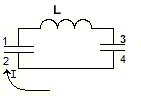
\includegraphics[height=30mm]{3_123.jpg}\\
	$\varphi_3 - \varphi_1 = L \der{q}{t}{2}$\\
	$\varphi_2 - \varphi_4 = 0$\\\\
	$-(\varphi_3 - \varphi_4) + (\varphi_1 - \varphi_2) = \frac{q_1}{C} - \frac{Q - q_1}{C} = - L \der{q_1}{t}{2}$\\
	$Q = C U_0 \quad \der{q_1}{t}{2} + 2 \frac{2}{LC} q_1 = \frac{Q}{LC} = \frac{U_0}{L}$\\
	$\assume q_1 = \tilde q_1 + C_1 \quad \der{q_1}{t}{2} + \frac{2}{LC} \tilde q = \frac{U_0}{L} - \frac{2 C_1}{LC} \Rightarrow C_1 \frac{CU_0}{2}$\\
	$q_1(0) = C U_0 \Rightarrow q_1(t) = \frac{C U_0}{2} (1 + \cos \omega t), \quad \omega = \sqrt{\frac{2}{LC}}$\\
	$q_2 = C U_0 - q_1 = \frac{CU_0}{2} (1 - \cos \omega t)$\\
}

